\documentclass[11pt, letterpaper]{article}

\usepackage{csquotes}	% Recommended?
\usepackage{xcolor}		% color
\usepackage{subfigure}	% subfigure
\usepackage{graphicx}
\usepackage{amssymb}	% symbol
\newcommand{\handout}[5]{
  \noindent
  \begin{center}
  \framebox{
    \vbox{
      \hbox to 5.78in { {\bf } \hfill #2 }
      \vspace{4mm}
      \hbox to 5.78in { {\Large \hfill #5  \hfill} }
      \vspace{2mm}
      \hbox to 5.78in { {\em #3 \hfill #4} }
    }
  }
  \end{center}
  \vspace*{4mm}
}
\newcommand{\lecture}[4]{\handout{#1}{#2}{#3}{#4}{#1}}

\newtheorem{theorem}{Theorem}
\newtheorem{corollary}[theorem]{Corollary}
\newtheorem{lemma}[theorem]{Lemma}
\newtheorem{observation}[theorem]{Observation}
\newtheorem{proposition}[theorem]{Proposition}
\newtheorem{definition}[theorem]{Definition}
\newtheorem{claim}[theorem]{Claim}
\newtheorem{fact}[theorem]{Fact}
\newtheorem{assumption}[theorem]{Assumption}
\topmargin 0pt
\advance \topmargin by -\headheight
\advance \topmargin by -\headsep
\textheight 9.5in
\oddsidemargin 0pt
\evensidemargin \oddsidemargin
\marginparwidth 0.5in
\textwidth 6.5in

\parindent 0in
\parskip 1.5ex

\begin{document}
\lecture{Programming Assignment 1 - Unfolding heuristics}{Spring 2016}{Yunjoo Park}{Computer Aided 3D Artifact Fabrication}


\section{Unfolding polytope}
Let \textit{P} be a polytope, bounded polyhedron. A simple polygon without overlapping is called \textit{net N} of \textit{P}. Each of polyhedra has multiple nets. The set of cut edges for the net is a spanning tree \textit{T}, the \textit{cut tree}, of \textit{G(P)}. An \textit{unfolding} is an isometric mappig \O : $F(P) \to {\mathbb{R}}^2 $ of the facets of $P$ to the Euclidean plane, such that for all $(f_1,f_2) \in D(P), \varphi(f_1)\cap \varphi(f_2)$ is an edge of both $\varphi(f_1)$ and $\varphi(f_2)$. $N(P,T) = \varphi(F(P))$ is the unfolding of \textit{P induced by T}. In this project, I will provide two implementation of unfolding heuristics from `Schlickenrieder, Wolfram. ``Net of Polyhedra." Master's Thesis, Technishe Universit$\ddot{a}$t Berlin (1997)' \cite{netpolyhedra}.
%In fact, there are two types of unfoldings. One is \textit{Edge unfolding}: Cut only along edges. The other is \textit{General unfoldings}: Cut through faces too. In this paper, I implement edge unfolding.
\section{The expected results}

\begin{enumerate}
	\item Source code for generating support materials		\textcolor{red}{$34\%$}
	\item Report contains the details of algorithm generating support materials	\textcolor{red}{$33\%$}
	\item The physical copies of the digital shadow art using a consumer-level 3D printer  \textcolor{red}{$33\%$} 2 of 5
    \begin{enumerate}
        \item jockey on horse using hands
        \item Dinasour with tools
        \item Musician playing a instrument using various instruments
    	\item something using pockemon
        \item disney castle using disney characters
	\end{enumerate}
\end{enumerate}

\section{Figures}
Following figures show expected results.

\begin{figure*}[th]
\centering
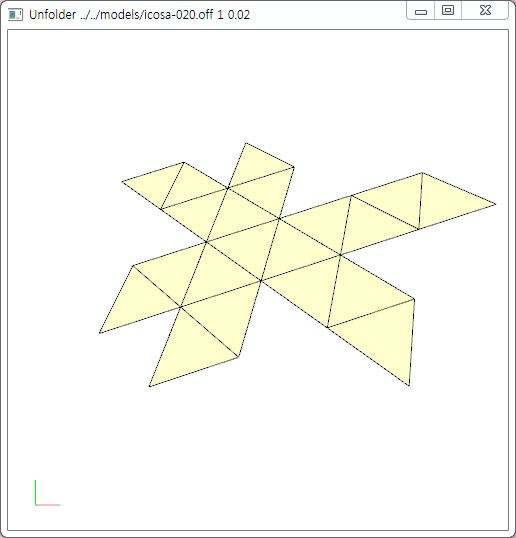
\includegraphics[width=0.6\textwidth]{FIGS/icosa-020.jpg}
\caption{Jockey on horse using hands}
\label{fig:jocky-on-horse}
\end{figure*}

\begin{figure*}[th]
\centering
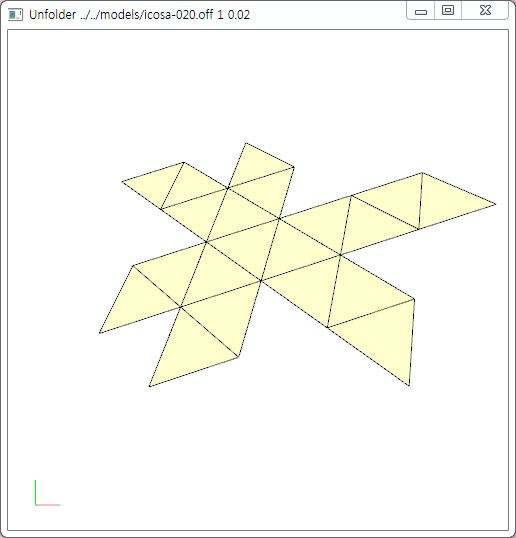
\includegraphics[width=0.6\textwidth]{FIGS/icosa-020.jpg}
\caption{Dinasour using tools}
\label{fig:dinasour}
\end{figure*}

\begin{figure*}[th]
\centering
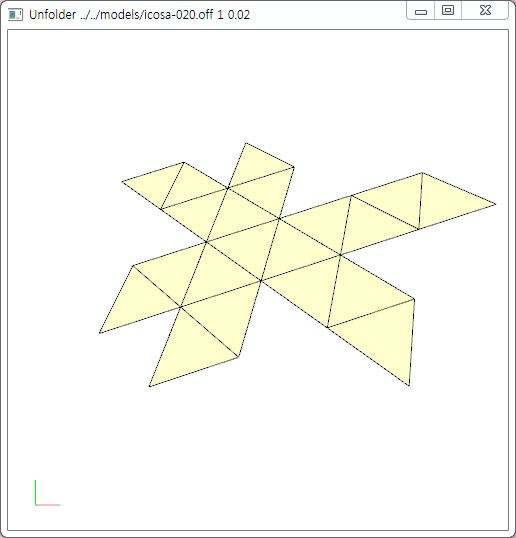
\includegraphics[width=0.6\textwidth]{FIGS/icosa-020.jpg}
\caption{Musicians playing instruments}
\label{fig:musicians}
\end{figure*}
    
\begin{figure*}[th]
\centering
{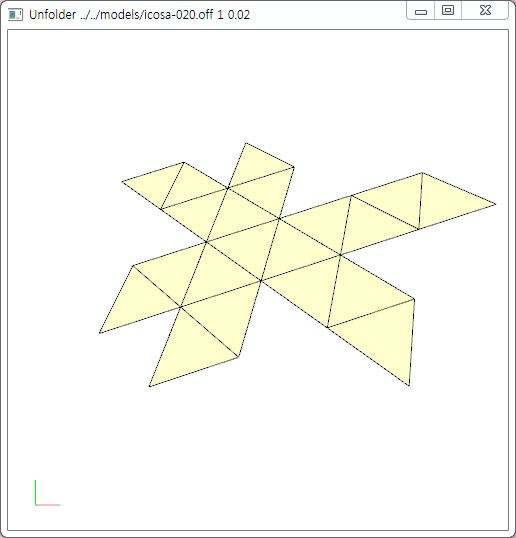
\includegraphics[height=0.22\textwidth]{FIGS/icosa-020.jpg}}\hfill
{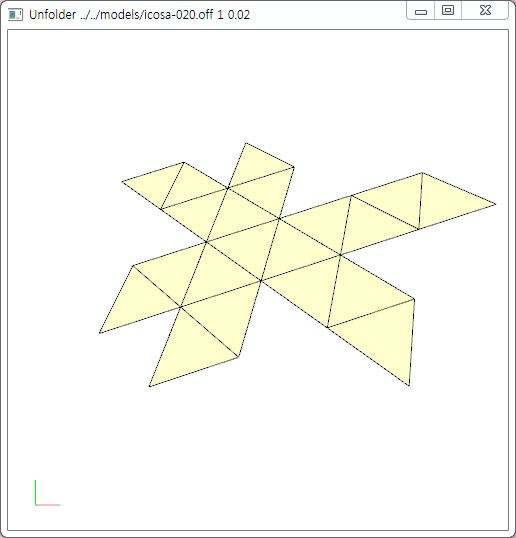
\includegraphics[height=0.22\textwidth]{FIGS/icosa-020.jpg}}\hfill
{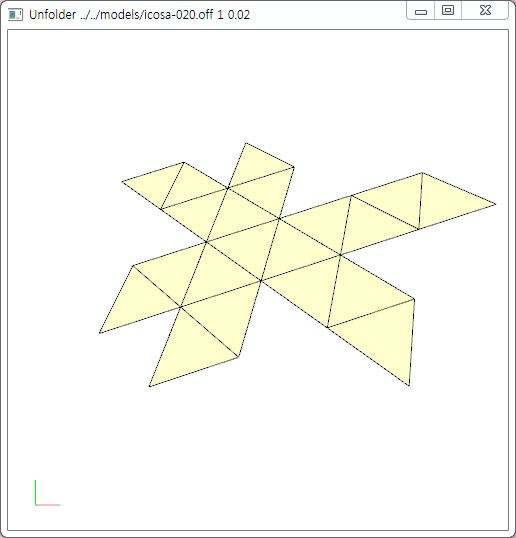
\includegraphics[height=0.22\textwidth]{FIGS/icosa-020.jpg}}\hfill
{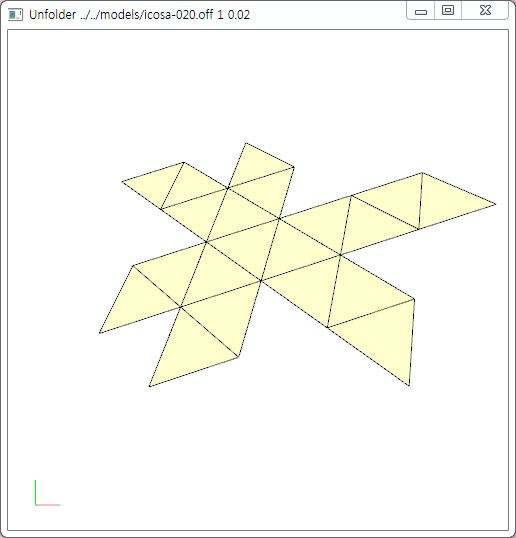
\includegraphics[height=0.22\textwidth]{FIGS/icosa-020.jpg}}\hfill
\caption{Pockemon silhouette}
\label{fig:pockemon}
\end{figure*}

\begin{figure*}[th]
\centering
\subfigure[target shadow]{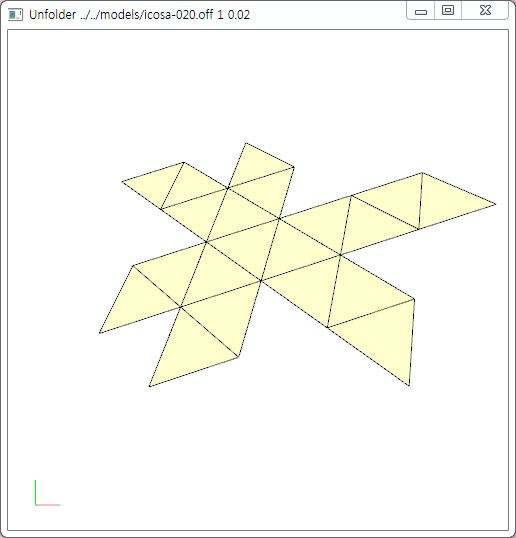
\includegraphics[width=0.22\textwidth]{FIGS/icosa-020.jpg}}\

\subfigure[stitch]
{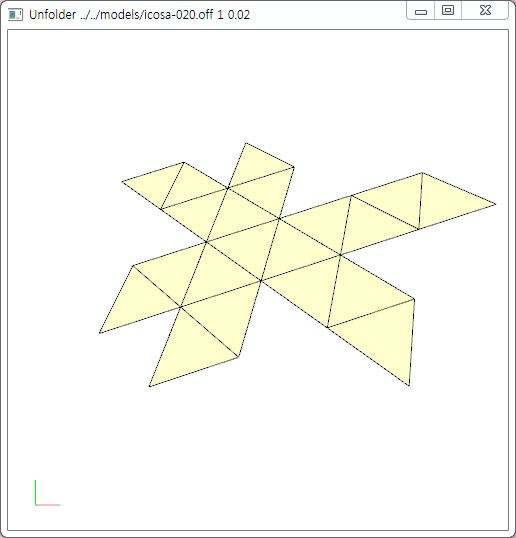
\includegraphics[height=0.22\textwidth]{FIGS/icosa-020.jpg}}\hfill
\subfigure[tinker bell]
{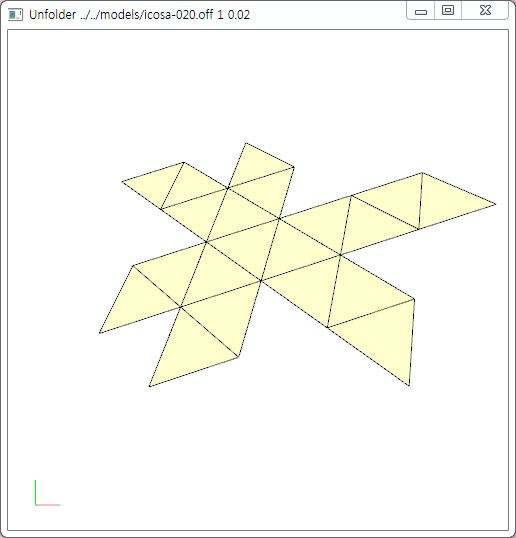
\includegraphics[height=0.22\textwidth]{FIGS/icosa-020.jpg}}\hfill
\subfigure[pooh]
{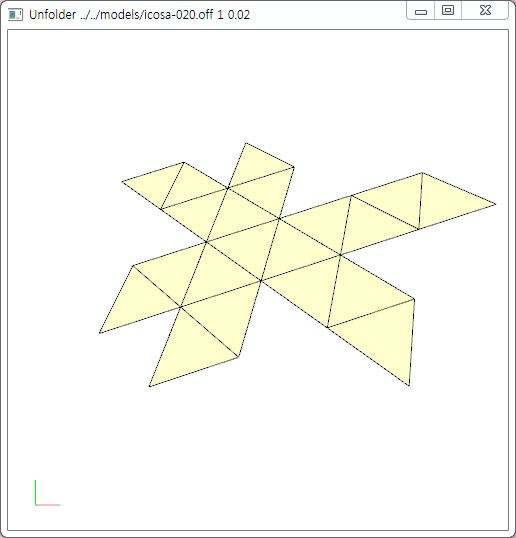
\includegraphics[height=0.22\textwidth]{FIGS/icosa-020.jpg}}\hfill
\subfigure[pluto]
{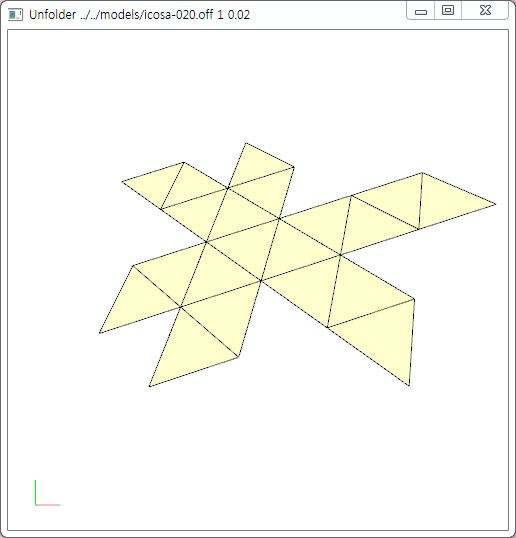
\includegraphics[height=0.22\textwidth]{FIGS/icosa-020.jpg}}\hfill
\subfigure[micky]
{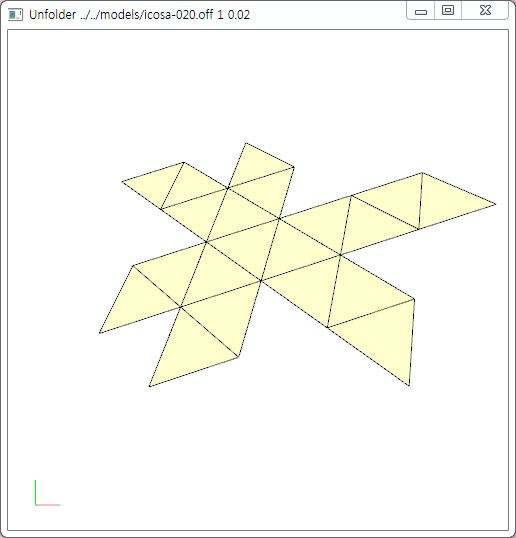
\includegraphics[height=0.22\textwidth]{FIGS/icosa-020.jpg}}\hfill

\caption{Disneyland castle silhouette and disney characters.}
\label{fig:disney}
\end{figure*}




%\printbibliography

\bibliographystyle{plain}
\bibliography{report}   % name your BibTeX data base
\end{document}